\section{Introdução}
\bibliographystyle{plainnat}

\subsection{Desafios}
\begin{frame}\frametitle{Introdução}

  \begin{tabular}{cc}  
    \begin{tabular}{c}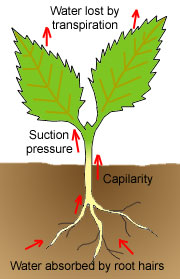
\includegraphics[height=3.5cm]{transp}\end{tabular} & 
  \begin{tabular}{c}\parbox{0.5\linewidth}{Desenvolvimento e produção \\ \centering{$\equiv$} \\ transpiração da planta}\end{tabular}  
    \\
    \begin{tabular}{c}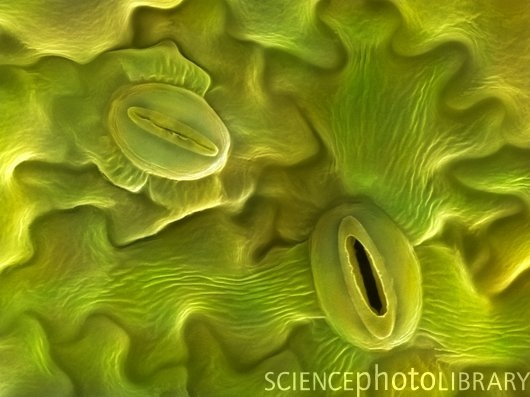
\includegraphics[height=2cm]{stomata}\end{tabular} &
  \begin{tabular}{c}\parbox{0.5\linewidth}{
      Estresse (biótico/abiótico) \\ \centering{$\downarrow$} \\ Fechamento dos estômatos \\ $\downarrow$ \\ Alteração na transpiração
  }\end{tabular} 
    \\
\end{tabular}
\end{frame}

\subsection{Soluções existentes}
\begin{frame}
  Revisão dos modelos existentes (inclusive o do Quirijn)
\end{frame}

\subsection{Solução proposta}
\begin{frame}
  Modelo proposto. Explicação de como funciona e caracterização.
\end{frame}

\subsection{Desafios da modelagem}
\begin{frame}\frametitle{Introdução}
  \begin{itemize}
    \item Encontrar um modelo que explique suficientemente bem o fenomeno para o propósito escolhido;
    \item Relação número de parâmetros/grau de complexidade do modelo difícil de ser ajustado;
    \item Encontrar simplificações que tornem a resolução possível, perdendo o mínimo possível de precisão \\ (realidade X simulação). \\~\\
  \end{itemize}
  \centering{Modelagem $\rightarrow$ entender/simular/prever os fenômenos \\ $\downarrow$ \\ melhorar práticas de manejo das culturas}
\end{frame}

%\subsection{Importância da modelagem}
%\begin{frame}\frametitle{Introdução}
%  \centering{Modelagem $\rightarrow$ entender/simular/prever os fenômenos \\ $\downarrow$ \\ melhorar práticas de manejo das culturas}
%\end{frame}

\subsection{Objetivos}
\begin{frame}
  %\frametitle{Objetivos da Tese}
  Os objetivos da tese são
  \begin{itemize}
  \item Incorporar extração de soluto no modelo de \cite{liersolute};
  \item Diferenciar quantitativamente as componentes passiva e ativa da extração de solutos;
  \end{itemize}
\end{frame}


